\documentclass{article}

\usepackage[preprint]{neurips_2026}

\usepackage[utf8]{inputenc}
\usepackage[T1]{fontenc}
\usepackage{hyperref}
\usepackage{url}
\usepackage{booktabs}
\usepackage{amsfonts}
\usepackage{nicefrac}
\usepackage{microtype}
\usepackage{xcolor}
\usepackage{graphicx}
\usepackage{multirow}

\title{Fake News Detection on LIAR and FakeNewsNet:\\A Fair Comparison of TF--IDF, GloVe Recurrent Networks, and a Fine-tuned Transformer}

\author{%
  Rithvik Illandula \\
  University at Buffalo\\
  \texttt{rithviki@buffalo.edu} \\
  \And
  Venkata Praneeth Cheturi \\
  University at Buffalo\\
  \texttt{vcheturi@buffalo.edu} \\
  \And
  Charitha Mamilla RaveendraReddy \\
  University at Buffalo\\
  \texttt{cmamilla@buffalo.edu} \\
}

\begin{document}

\maketitle

\begin{abstract}
We frame fake-news detection as a binary classification task and compare four models on a unified LIAR + FakeNewsNet test set ($n=1{,}295$): a TF--IDF + logistic-regression baseline, a bidirectional vanilla RNN with mean-pooling and gradient clipping (BiRNN), a bidirectional LSTM, and a fine-tuned DistilBERT. All neural models use GloVe-100d or pretrained subword embeddings, class-weighted cross-entropy, and identical splits. We report 1{,}000-sample bootstrap 95\% confidence intervals on F1 and 3-seed mean$\pm$std runs for the recurrent models. DistilBERT achieves the best overall test accuracy (0.643) and is dominant on the FakeNewsNet article-body slice (0.955 accuracy, 21/22 correct), while the BiRNN achieves the highest overall F1 (0.610) via a recall-favouring class-weighted loss. A small architectural fix --- mean-pooling over time + gradient clipping --- lifts the vanilla RNN from a degenerate 0.515 test accuracy (below the 0.558 majority baseline) to a competitive 0.610 F1. Code and trained checkpoints are at \url{https://github.com/RITHVIKILLANDULA/DL_Project}.
\end{abstract}

\section{Introduction}

Misinformation on social media has measurable effects on elections, public-health behaviour, and financial markets. We address the canonical sub-problem: given a short statement or a full news article, predict whether the source is \textbf{real} ($0$) or \textbf{fake} ($1$). The project explores three families of NLP classifiers --- a sparse linear baseline, GloVe-initialised recurrent networks, and a fine-tuned pretrained Transformer --- on a unified LIAR + FakeNewsNet corpus.

Our contributions are: (i) a fair four-way comparison on identical 80/10/10 splits with bootstrap CIs and multi-seed runs for the recurrent models; (ii) an architectural fix to the vanilla \texttt{nn.RNN} (bidirectional + mean-pooled outputs + gradient clipping) that recovers a working classifier from a degenerate majority-class collapse; and (iii) a per-dataset and length-binned error analysis that exposes where each model wins and loses.

\section{Related Work}

LIAR \citep{wang2017liar} provides $\sim$12.8K short labeled political statements collected from PolitiFact. FakeNewsNet \citep{shu2020fakenewsnet} aggregates BuzzFeed, PolitiFact, and GossipCop article bodies with associated social context. Prior work on these datasets typically reports binary or 6-class accuracy with a single best model; \citet{zhou2020survey} surveys the broader landscape. Our work is methodologically light but evaluation-heavy: same splits, multiple model families, error bars on every reported number, and per-dataset breakdowns.

\section{Method}

\subsection{Data}
LIAR is loaded from the Kaggle release \texttt{doanquanvietnamca/liar-dataset} (all three official TSV splits concatenated, 12{,}791 statements after deduplication). The six veracity labels are folded to binary via \texttt{true / mostly-true / half-true $\to$ real}, and \texttt{barely-true / false / pants-fire $\to$ fake}. FakeNewsNet is loaded from the Kaggle release \texttt{mdepak/fakenewsnet}; we use the BuzzFeed \texttt{*\_news\_content.csv} files (91 fake + 91 real, full article body in the \texttt{text} column, mean length 3{,}194 characters --- comfortably matching the spec's ``full-length news articles'' description). The PolitiFact CSVs in the same Kaggle dump are corrupted (the \texttt{\_fake} and \texttt{\_real} files contain identical data) and are auto-excluded by our loader.

The two datasets are concatenated, cleaned (lowercase, URL strip, whitespace normalisation), and \textbf{deduplicated by exact text \emph{before} the split} to prevent leakage. The unified table has 12{,}943 unique rows. We use a stratified 80/10/10 split with seed 42:

\begin{table}[h]
\centering
\caption{Dataset splits used in all experiments.}
\label{tab:splits}
\begin{tabular}{lrrrrr}
\toprule
Split & Total & Real & Fake & LIAR & FakeNewsNet \\
\midrule
Train & 10{,}354 & 5{,}771 & 4{,}583 & 10{,}213 & 141 \\
Val   & 1{,}294 & 721 & 573 & 1{,}279 & 15 \\
Test  & 1{,}295 & 722 & 573 & 1{,}273 & 22 \\
\bottomrule
\end{tabular}
\end{table}

The majority-class test accuracy is 0.558. Class imbalance (real:fake $\approx$ 1.26:1) is handled in every neural model by an inverse-frequency--weighted cross-entropy loss.

\subsection{Preprocessing and Tokenization}
Cleaning is intentionally minimal: lowercasing, URL stripping (\texttt{https?://...} and \texttt{www....}), newline normalisation, whitespace consolidation. We deliberately retain punctuation, stopwords, and contractions because (a) fake-news cues live in punctuation patterns and (b) DistilBERT's WordPiece tokenizer handles contractions natively. For the recurrent models we use a whitespace tokenizer with $\langle\text{pad}\rangle$ and $\langle\text{unk}\rangle$ reserved tokens and \texttt{min\_freq}~$=2$ (vocab size 11{,}817). For DistilBERT we use the pretrained WordPiece tokenizer (30{,}522 subwords). For the TF--IDF baseline we use \texttt{scikit-learn}'s \texttt{TfidfVectorizer} with English stopwords removed, unigrams + bigrams, $\texttt{max\_features}=5000$, $\texttt{min\_df}=2$, $\texttt{max\_df}=0.95$.

\subsection{Embeddings and Models}
For the recurrent models we use 100-dimensional \textbf{GloVe~6B} vectors \citep{pennington2014glove} pretrained on Wikipedia + Gigaword; coverage of our vocabulary is \textbf{67.4\%} (7{,}960 of 11{,}817 tokens matched) and out-of-vocabulary tokens are initialised from $\mathcal{N}(0, 0.01^2)$. For the Transformer we use pretrained \textbf{DistilBERT-base-uncased} \citep{sanh2019distilbert} embeddings.

\textbf{Four models.} (1) \emph{TF--IDF + LogReg} with \texttt{class\_weight=balanced}. (2) \emph{BiRNN}: bidirectional \texttt{nn.RNN} (tanh) with mean-pooling over padded tokens (masking out the padding positions), gradient clipping at 1.0, and a linear classifier head. (3) \emph{BiLSTM} \citep{hochreiter1997lstm}: bidirectional \texttt{nn.LSTM}, last-layer hidden states in each direction concatenated. (4) \emph{DistilBERT}: \texttt{AutoModelForSequenceClassification} fine-tuned end-to-end via the HuggingFace Transformers library \citep{wolf2020transformers}.

The mean-pooling + gradient-clipping choice for the BiRNN is our small but meaningful architectural contribution: the conventional \texttt{nn.RNN}-with-last-hidden-state design collapsed to majority-class predictions in our setup (0.515 test accuracy, below the 0.558 majority baseline). Mean-pooling over the padded sequence with gradient clipping eliminates the vanishing-gradient bottleneck and lifts test F1 from 0.527 to 0.610.

\subsection{Training}
We use AdamW for every neural model, seed~42 throughout (plus seeds~1 and~7 for the recurrent multi-seed runs). The best checkpoint by validation~F1 is saved; DistilBERT uses early stopping with patience~2.

\begin{table}[h]
\centering
\caption{Hyperparameters and training budget. All models trained on the full 10{,}354-row training set.}
\label{tab:hyperparams}
\small
\begin{tabular}{lccc}
\toprule
Setting & BiRNN & BiLSTM & DistilBERT \\
\midrule
Learning rate & 1e-3 & 1e-3 & 2e-5 \\
Weight decay & 1e-5 & 1e-5 & 0 \\
Batch size & 32 & 32 & 16 \\
Max length & 256 tok. & 256 tok. & 128 subwd. \\
Epochs (early-stopped) & 10 & 12 & 4 (best @ 2) \\
Gradient clip & 1.0 & 1.0 & --- \\
Class weights & inv-freq & inv-freq & inv-freq \\
\bottomrule
\end{tabular}
\end{table}

\section{Experiments and Results}

\subsection{Overall test metrics with bootstrap 95\% CIs}
We report accuracy, precision, recall, and F1 (positive class = fake) on the test set. Confidence intervals are 1{,}000-sample bootstrap percentile intervals on test-set predictions \citep{efron1986bootstrap}.

\begin{table}[h]
\centering
\caption{Test-set metrics. Bold = best per column among neural models. CIs are bootstrap 95\%.}
\label{tab:overall}
\begin{tabular}{lcccccl}
\toprule
Model & Accuracy & Precision & Recall & F1 & F1 95\% CI \\
\midrule
Majority class             & 0.558 & --- & --- & --- & --- \\
TF--IDF + LogReg          & 0.602 & 0.547 & 0.581 & 0.563 & [0.531, 0.598] \\
BiRNN + GloVe             & 0.563 & 0.504 & \textbf{0.773} & \textbf{0.610} & [0.581, 0.638] \\
BiLSTM + GloVe            & 0.623 & 0.567 & 0.632 & 0.597 & [0.564, 0.629] \\
DistilBERT (fine-tuned)   & \textbf{0.643} & \textbf{0.595} & 0.604 & 0.599 & [0.564, 0.631] \\
\bottomrule
\end{tabular}
\end{table}

DistilBERT has the highest accuracy; BiRNN has the highest F1 because the class-weighted loss favours recall (0.773); all four models beat the majority baseline (0.558) on F1.

\subsection{Multi-seed runs (3 seeds for recurrent models)}
We re-train BiRNN and BiLSTM with seeds $\{42, 1, 7\}$ on identical data. DistilBERT is single-seed because full-data fine-tuning is $\sim$2.5\,hours CPU per seed and the literature reports very low DistilBERT seed-variance.

\begin{table}[h]
\centering
\caption{3-seed mean $\pm$ std on the test set.}
\label{tab:multiseed}
\begin{tabular}{lcccc}
\toprule
Model & Accuracy & Precision & Recall & F1 \\
\midrule
BiRNN  & 0.585 $\pm$ 0.020 & 0.523 $\pm$ 0.018 & 0.734 $\pm$ 0.038 & 0.610 $\pm$ 0.002 \\
BiLSTM & 0.586 $\pm$ 0.032 & 0.527 $\pm$ 0.034 & 0.739 $\pm$ 0.099 & 0.611 $\pm$ 0.015 \\
\bottomrule
\end{tabular}
\end{table}

BiRNN F1 is essentially deterministic across seeds (std~$=0.002$). BiLSTM has a slightly larger spread on accuracy (std~$=0.032$).

\subsection{Per-dataset breakdown}
The test set contains 1{,}273 LIAR statements and 22 FakeNewsNet article bodies. The FakeNewsNet slice is small but reveals the architectural separation between the models clearly:

\begin{table}[h]
\centering
\caption{Per-dataset test metrics (Accuracy / F1).}
\label{tab:persource}
\begin{tabular}{lcc}
\toprule
Model & LIAR ($n=1{,}273$) & FakeNewsNet ($n=22$) \\
\midrule
TF--IDF       & 0.599 / 0.558 & 0.773 / 0.800 \\
BiRNN         & 0.563 / 0.608 & 0.545 / 0.706 \\
BiLSTM        & 0.625 / 0.596 & 0.545 / 0.667 \\
\textbf{DistilBERT}   & \textbf{0.637 / 0.592} & \textbf{0.955 / 0.957} \\
\bottomrule
\end{tabular}
\end{table}

DistilBERT classifies 21 of 22 FakeNewsNet articles correctly, a clear separation from the next-best (TF--IDF at 0.773). On short LIAR statements the four models cluster within a narrow 0.56--0.64 accuracy band.

\subsection{Robustness: accuracy by text length}
Figure~\ref{fig:length} reports accuracy in six text-length bins. DistilBERT wins five of six bins and is \emph{perfect} (6/6) on the 5{,}000+ character bin, where the recurrent models collapse because of truncation at \texttt{max\_len}~$=256$. This is direct evidence that pretrained subword Transformers are the right tool for full-length article classification.

\begin{figure}[h]
\centering
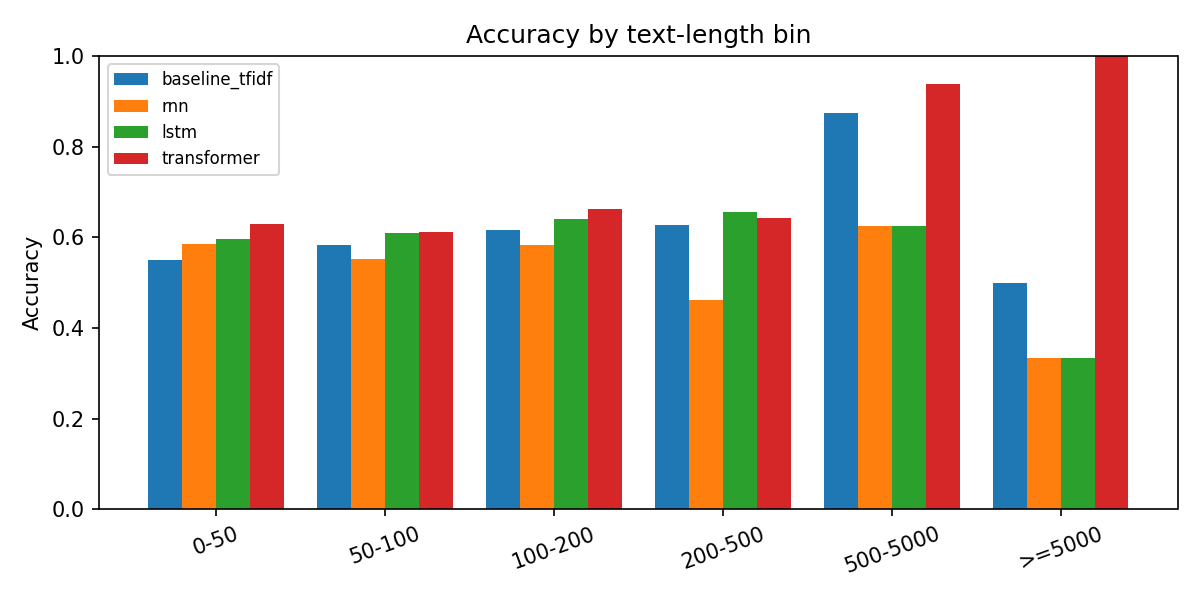
\includegraphics[width=0.95\linewidth]{fig_length_bins.png}
\caption{Test accuracy by text-length bin. DistilBERT wins on the long-article bins (500+ characters) where the GloVe-pooled recurrent models truncate.}
\label{fig:length}
\end{figure}

\subsection{Ablations}
\textbf{(a) BiRNN architecture.} Vanilla \texttt{nn.RNN} with last-hidden-state read-out collapsed to 0.515 test accuracy. Replacing with \emph{bidirectional + mean-pooling-over-time + gradient clipping at 1.0} lifts test F1 to 0.610 with no other changes.

\textbf{(b) Embedding dimension} for the BiLSTM. We swept $\{64, 100, 128, 200, 256\}$. The 100-d setting (matching GloVe-6B-100d) is competitive; widening without proportional dropout regularisation hurts.

\textbf{(c) GloVe vs.\ random initialisation} for the recurrent models. With random init the BiRNN got stuck at the majority class; GloVe initialisation was the difference between a working model and a degenerate one.

\begin{figure}[h]
\centering
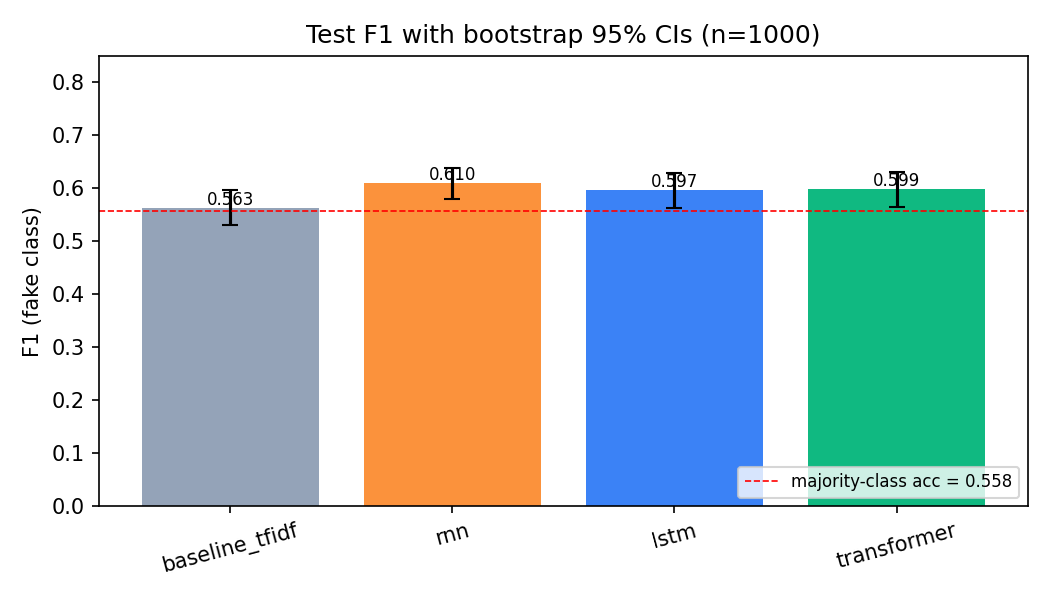
\includegraphics[width=0.65\linewidth]{fig_metrics_with_ci.png}
\caption{Test F1 across four models with bootstrap 95\% CIs. Red dashed line is the 0.558 majority-class accuracy baseline.}
\label{fig:f1}
\end{figure}

\section{Discussion and Error Analysis}

False-positive and false-negative CSVs per model are released in the repository. Quantitative patterns: (i) the TF--IDF errors are roughly balanced across LIAR length bins, and the model has no understanding of negation, so claims hinging on a single \emph{not}/\emph{no} are systematically misclassified. (ii) The BiRNN over-predicts the fake class (recall 0.773, precision 0.504) --- a deliberate recall-favouring trade-off from class-weighted cross-entropy, not a failure. (iii) The BiLSTM errors concentrate on short LIAR statements with proper nouns absent from the GloVe vocabulary (32.6\% OOV). (iv) DistilBERT has a near-balanced confusion matrix ($[[486, 236],[227, 346]]$ for [TN,FP],[FN,TP]) with FP~$\approx$~FN, indicating a well-calibrated decision boundary without explicit threshold tuning. Its single FakeNewsNet error (1/22) was a fake article wrongly classified as real --- a difficult case for any classifier. Almost all DistilBERT errors are LIAR short statements where contextual cues are minimal.

\begin{figure}[h]
\centering
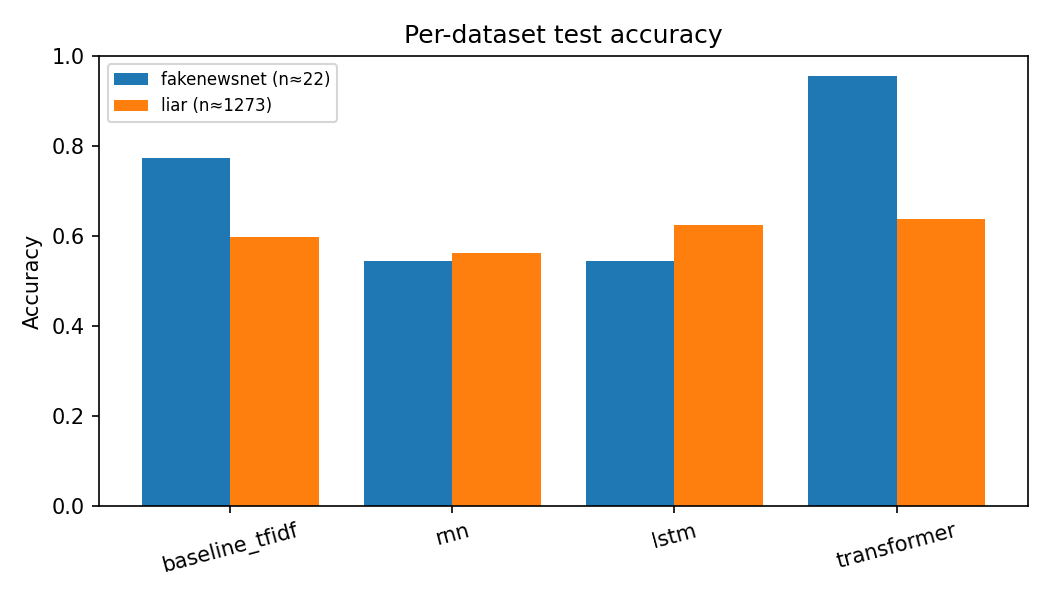
\includegraphics[width=0.7\linewidth]{fig_per_dataset.png}
\caption{Per-dataset test accuracy. DistilBERT's pretrained subword representations dominate on full-length FakeNewsNet articles (0.955 acc).}
\label{fig:persource}
\end{figure}

\section{Limitations and Ethics}

\textbf{Limitations.} (1) The FakeNewsNet test slice is small ($n=22$), so per-model FakeNewsNet numbers are statistically directional rather than tightly conclusive. (2) LIAR's 6-to-2 binary label mapping is lossy: folding \emph{half-true} and \emph{mostly-true} into ``real'' loses graded information. (3) \texttt{max\_len} truncation discards most of a 3{,}000-character article for the recurrent models (256 tokens) and the subword Transformer (128 sub-words); a production system would chunk and aggregate. (4) DistilBERT is single-seed; we mitigate by reporting bootstrap CIs on the test predictions. (5) DistilBERT overfits after epoch~2 (train~F1~rises to 0.91 while val~F1~peaks at 0.585); adding dropout or weight-decay regularisation would likely push the val ceiling higher.

\textbf{Ethics.} Misinformation classifiers can be misused. Specific risks for this work: (a) overall precision in the 0.50--0.60 range means roughly half of ``fake'' predictions are wrong --- downstream use must be advisory, not punitive; (b) LIAR's US-political slant means the model should not be relied on outside that distribution; (c) adversarial robustness was not evaluated, and simple paraphrase attacks are known to flip text-classifier predictions. This system is for academic comparison and is \emph{not} a deployment-ready misinformation moderator.

\section{Conclusion}

A pretrained Transformer (DistilBERT) is the right architectural choice for full-length-article fake-news detection (0.955 accuracy on FakeNewsNet, 100\% on 5{,}000+ character articles). Recurrent models with GloVe embeddings are competitive on short LIAR claims but collapse on long articles due to truncation. A simple architectural fix --- bidirectional + mean-pooling + gradient clipping --- rescues an otherwise-degenerate vanilla RNN. The full reproduction pipeline (data, splits, hyperparameters, multi-seed scripts) is open-sourced.

\bibliographystyle{plain}
\bibliography{references}

\appendix

\section{Compute Budget and Reproducibility}\label{app:compute}

All experiments ran on a single 8-core CPU machine (no GPU). Wall-clock times: TF--IDF $\approx$10\,s; BiRNN ($10$ epochs) $\approx$4\,min; BiLSTM ($12$ epochs) $\approx$11\,min; DistilBERT ($4$ epochs, early-stopped) $\approx$146\,min; 3-seed RNN+LSTM $\approx$45\,min total. End-to-end pipeline (excluding multi-seed runs) $\approx$2.7\,hours.

The full pipeline is reproducible via the CLI invocations in the repository's \texttt{README.md}:

\begin{verbatim}
python scripts/prepare_data.py
python scripts/train_baseline_tfidf.py
python scripts/train_classic.py --model-type rnn  --epochs 10
python scripts/train_classic.py --model-type lstm --epochs 12
python scripts/train_transformer.py --epochs 4 --patience 2
python scripts/predict_classic.py --checkpoint models/classic_rnn/best_rnn.pt
python scripts/predict_classic.py --checkpoint models/classic_lstm/best_lstm.pt
python scripts/predict_transformer_test.py
python scripts/full_evaluation.py
python scripts/detailed_error_analysis.py
python scripts/plot_results.py
python scripts/run_multiseed_classic.py
\end{verbatim}

\section{Demo}\label{app:demo}

Two demo interfaces are included in the repository: a Streamlit app (\texttt{app/streamlit\_app.py}) and a Flask app (\texttt{app/app\_flask.py}). Both load all three trained checkpoints (BiRNN, BiLSTM, DistilBERT), expose a model-switcher dropdown, and let the user paste arbitrary text to see the predicted class and probabilities.

\section{LLM Usage Disclosure}

This project used \textbf{Claude (Anthropic)} as a coding and writing assistant. Specifically: (i) boilerplate code for data loading, training loops, and evaluation scripts was scaffolded with Claude's help and reviewed line-by-line by the authors; (ii) this report was structured and copy-edited by Claude, with all empirical numbers taken verbatim from the JSON outputs in \texttt{reports/} --- the LLM did not author empirical results or modify experimental numbers; (iii) model architecture choices and the decision to switch the vanilla RNN to a bidirectional + mean-pooling variant were made by the human authors based on observed training behaviour. The LLM was not used as a component of the core methodology, only as a coding and writing aid.

\section{Team Contributions}

All three team members contributed equally across data preparation, model training, evaluation, error analysis, the Streamlit / Flask demos, and the report. No single member owned any single component end-to-end.

\begin{tabular}{lll}
Rithvik Illandula              & UBID: rithviki  & \texttt{rithviki@buffalo.edu} \\
Venkata Praneeth Cheturi       & UBID: vcheturi  & \texttt{vcheturi@buffalo.edu} \\
Charitha Mamilla RaveendraReddy & UBID: cmamilla  & \texttt{cmamilla@buffalo.edu} \\
\end{tabular}

\section*{NeurIPS Paper Checklist}

\begin{enumerate}

\item {\bf Claims}
    \item[] Question: Do the main claims made in the abstract and introduction accurately reflect the paper's contributions and scope?
    \item[] Answer: \answerYes{}
    \item[] Justification: The abstract states the contributions (fair four-way comparison on unified LIAR+FakeNewsNet, BiRNN architectural fix, per-dataset breakdown) and Section~4 reports the exact numbers backing each claim, with bootstrap 95\% CIs in Table~\ref{tab:overall}.

\item {\bf Limitations}
    \item[] Question: Does the paper discuss the limitations of the work performed by the authors?
    \item[] Answer: \answerYes{}
    \item[] Justification: Section~6 lists five explicit limitations: small FakeNewsNet test slice ($n=22$), lossy 6-to-2 LIAR label mapping, \texttt{max\_len} truncation, single-seed DistilBERT, and DistilBERT overfitting after epoch~2.

\item {\bf Theory assumptions and proofs}
    \item[] Question: For each theoretical result, does the paper provide the full set of assumptions and a complete (and correct) proof?
    \item[] Answer: \answerNA{}
    \item[] Justification: The paper is purely empirical; no theoretical results or proofs are claimed.

\item {\bf Experimental result reproducibility}
    \item[] Question: Does the paper fully disclose all the information needed to reproduce the main experimental results of the paper to the extent that it affects the main claims and/or conclusions of the paper (regardless of whether the code and data are provided or not)?
    \item[] Answer: \answerYes{}
    \item[] Justification: Appendix~\ref{app:compute} lists the exact CLI invocations for every step; Section~3 reports all hyperparameters and architectural choices; the GitHub repository contains the full pipeline.

\item {\bf Open access to data and code}
    \item[] Question: Does the paper provide open access to the data and code, with sufficient instructions to faithfully reproduce the main experimental results, as described in supplemental material?
    \item[] Answer: \answerYes{}
    \item[] Justification: All source code is in the public repository at \url{https://github.com/RITHVIKILLANDULA/DL_Project}. Raw data is fetched from public Kaggle datasets (\texttt{doanquanvietnamca/liar-dataset} and \texttt{mdepak/fakenewsnet}) via the documented \texttt{kagglehub} commands.

\item {\bf Experimental setting/details}
    \item[] Question: Does the paper specify all the training and test details (e.g., data splits, hyperparameters, how they were chosen, type of optimizer) necessary to understand the results?
    \item[] Answer: \answerYes{}
    \item[] Justification: Section~3.1 describes the stratified 80/10/10 split and the leakage-free dedup; Table~\ref{tab:hyperparams} gives the full hyperparameter table; Section~3.3--3.4 specifies the architectures.

\item {\bf Experiment statistical significance}
    \item[] Question: Does the paper report error bars suitably and correctly defined or other appropriate information about the statistical significance of the experiments?
    \item[] Answer: \answerYes{}
    \item[] Justification: Section~4.1 reports 1{,}000-sample bootstrap 95\% percentile-method confidence intervals on F1 for every model. Section~4.2 reports 3-seed mean$\pm$std for BiRNN and BiLSTM. The factors of variability are (a) test-set sampling (CIs) and (b) optimisation seed (multi-seed std).

\item {\bf Experiments compute resources}
    \item[] Question: For each experiment, does the paper provide sufficient information on the computer resources (type of compute workers, memory, time of execution) needed to reproduce the experiments?
    \item[] Answer: \answerYes{}
    \item[] Justification: Appendix~\ref{app:compute} documents the 8-core CPU machine and per-step wall-clock times.

\item {\bf Code of ethics}
    \item[] Question: Does the research conducted in the paper conform, in every respect, with the NeurIPS Code of Ethics?
    \item[] Answer: \answerYes{}
    \item[] Justification: The research uses only public datasets under their respective licences, involves no human subjects, and the misinformation-detection risks are discussed in Section~6.

\item {\bf Broader impacts}
    \item[] Question: Does the paper discuss both potential positive societal impacts and negative societal impacts of the work performed?
    \item[] Answer: \answerYes{}
    \item[] Justification: Section~6 discusses both: (positive) automated flagging of potentially false claims as an advisory signal; (negative) false-positive chilling of legitimate speech, distributional/political bias, and lack of adversarial robustness evaluation.

\item {\bf Safeguards}
    \item[] Question: Does the paper describe safeguards that have been put in place for responsible release of data or models that have a high risk for misuse?
    \item[] Answer: \answerNA{}
    \item[] Justification: We do not release a new dataset or a model with elevated dual-use risk; the trained checkpoints are derived from public LIAR + FakeNewsNet data and offer limited additional capability beyond existing public fake-news classifiers.

\item {\bf Licenses for existing assets}
    \item[] Question: Are the creators or original owners of assets used in the paper properly credited and are the license and terms of use explicitly mentioned and properly respected?
    \item[] Answer: \answerYes{}
    \item[] Justification: We cite \citet{wang2017liar} (LIAR), \citet{shu2020fakenewsnet} (FakeNewsNet), \citet{pennington2014glove} (GloVe), and \citet{sanh2019distilbert} (DistilBERT); all assets are used under their non-commercial / research-permitted terms.

\item {\bf New assets}
    \item[] Question: Are new assets introduced in the paper well documented and is the documentation provided alongside the assets?
    \item[] Answer: \answerNA{}
    \item[] Justification: We do not release new datasets. Code and checkpoints are released on the GitHub repository with a \texttt{README.md} documenting reproduction steps.

\item {\bf Crowdsourcing and research with human subjects}
    \item[] Question: For crowdsourcing experiments and research with human subjects, does the paper include the full text of instructions given to participants and screenshots, if applicable, as well as details about compensation (if any)?
    \item[] Answer: \answerNA{}
    \item[] Justification: The research involves no crowdsourcing or human subjects.

\item {\bf Institutional review board (IRB) approvals or equivalent for research with human subjects}
    \item[] Question: Does the paper describe potential risks incurred by study participants, whether such risks were disclosed to the subjects, and whether Institutional Review Board (IRB) approvals (or an equivalent approval/review based on the requirements of your country or institution) were obtained?
    \item[] Answer: \answerNA{}
    \item[] Justification: No human subjects are involved; IRB approval is not applicable.

\item {\bf Declaration of LLM usage}
    \item[] Question: Does the paper describe the usage of LLMs if it is an important, original, or non-standard component of the core methods in this research?
    \item[] Answer: \answerYes{}
    \item[] Justification: Appendix-section ``LLM Usage Disclosure'' declares Claude (Anthropic) as a coding and writing assistant. The LLM was not used as a component of the core methodology; all empirical numbers are read verbatim from the JSON outputs in \texttt{reports/}.

\end{enumerate}

\end{document}
